\documentclass[12pt,twoside]{article}
\usepackage[parfill]{parskip}  
\usepackage{graphicx}
\usepackage{amssymb}
\usepackage{amsmath}
\usepackage{epstopdf}
\usepackage{underscore}
\usepackage{caption}
\DeclareGraphicsRule{.tif}{png}{.png}{`convert #1 `dirname #1`/`basename #1 .tif`.png}
\usepackage{fourier}
\usepackage{listings}
\lstset{
	language=java,
	tabsize=4,
	frame=trbl,
	columns=fullflexible,
	escapechar=\#,
	basicstyle=\sffamily,
	stringstyle=\textit,
	showstringspaces=false}
\usepackage{pdfpages}
%\usepackage{pdfsync}
% from use-full-height.tex
\setlength{\textheight}{9.5in}
\setlength{\headheight}{.60in}
\setlength{\headsep}{.40in}
\setlength{\topmargin}{-1.5in}

% from use-full-width.tex
\setlength{\textwidth}{6.5in} 
\setlength{\oddsidemargin}{0in}
\setlength{\evensidemargin}{0in}

% crowd figures and text on pages to reduce page count
\renewcommand\floatpagefraction{.9}
\renewcommand\topfraction{.9}
\renewcommand\bottomfraction{.9}
\renewcommand\textfraction{.1}   
\setcounter{totalnumber}{50}
\setcounter{topnumber}{50}
\setcounter{bottomnumber}{50}

% use san-serif for code
\renewcommand{\ttdefault}{\sfdefault}

% ----------------------------------------------------------------
% Question formatting macros
% ----------------------------------------------------------------
\newcommand{\fillInBlank}[1][0.5in]{\underline{\hspace{#1}}}
\newcommand*{\fixme}[1]{\textsc{To be fixed:} \emph{{#1}}}

% #1 answer: T, F, or none to hide
% #2 question text
\newcommand*{\truefalse}[2][none]{\hspace{0.25in}%
\ifthenelse{\equal{#1}{none}}{T\hspace{0.15in}F}{%
	\ifthenelse{\equal{#1}{T}}{T\hspace{0.25in}}{%
		\hspace{0.25in}F}}%
\hspace{0.15in}{#2}}

\newcommand*{\bigoh}[1]{\ensuremath{\mathrm{O}({#1})}}

\newcommand*{\littleoh}[1]{\ensuremath{\mathrm{o}({#1})}}

\newcommand*{\bigtheta}[1]{\ensuremath{\Theta({#1})}}
% ----------------------------------------------------------------

\renewcommand{\labelenumi}{\alph{enumi}.}

\newcommand{\code}[1]{\texttt{#1}}

\frenchspacing

\begin{document}
%\maketitle

\begin{flushright}
Name: \fillInBlank[3in] Section: \fillInBlank[1in]

\LARGE{CSSE 220---Object-Oriented Software Development}

\Large{Exam 1 -- Part 2, Dec. 18, 2015}
\end{flushright}

\textbf{Allowed Resources on Part 2.} \hspace{0.15in}
Open book, open notes, and computer. Limited network access. You may use the network only to access your own files, the course Moodle and Piazza sites (but obviously don't post on Piazza) and web pages, the textbook's site, Oracle's Java website, and Logan Library's online books.


\textbf{Instructions}.\hspace{0.15in}
\emph{You must disable Microsoft Lync, IM, email, and other such communication programs before beginning part 2 of the exam. Any communication with anyone other than the instructor or a TA during the exam may result in a failing grade for the course.}

You must actually get these problems working on your computer. Almost all of the credit for the problems will be for code that actually works. There are several different small methods to write, so you can get a lot of partial credit by getting some of them to work.  If you get every part working, comments are not required.  If you do not get a method to work, comments may help me to understand enough so I can give you (a small amount of) partial credit.  

\textbf{Begin part 2 by checking out the project named \emph{Exam1-201620} from your course SVN repository}.  (Ask for help immediately if you are unable to do this.)

When you have finished a problem, and more frequently if you wish, \textbf{submit your code by committing it to your SVN repository}.  We will check commit logs, so you must be careful not to commit anything after the end of the exam.  For grading, we will ensure that the included JUnit tests have not been changed.

\emph{Part 2 is included in this document.}
\textbf{Do not use non--approved websites like search engines (Google) or any website other than those above.}  Be sure to turn in the these instructions, with your name written above, to your exam proctor. You should not exit the examination room with these instructions.

\clearpage
{\Large Part 2---Computer Part}

\vspace{0.25in}
\hrule
{\large Problem Descriptions}

\textbf{Part A: Small Problems} (24 points) Implement the code for the 3 functions in \code{SmallProblems.java} -- each problem is worth 8 points. Instructions are included in the comments of each function.  Unit tests are included in \code{SmallProblemsTest.java}.

\vspace{0.15in}

\textbf{Part B: Map and 2D Array Problems} (18 points) Implement the code for the functions in \code{MapAnd2dArray.java} -- each problem is worth 9 points.  Instructions are included in the comments of each function.  Unit tests are included in \code{MapAnd2DArrayTest.java}.

\vspace{0.15in}


\textbf{Part C: Test This Class} (6 points) Implement a unit test for the function in \code{TestThisClass.java}.  You will add a file \code{TestThisClassTest.java} that will contain your test.  Your test should have 3 assertions that test a variety of cases, but need not be exhaustive.

\vspace{0.15in}

\textbf{Part D on next page}

\clearpage

\textbf{Part D: Rectangles} (17 points) 

\begin{figure}
	\begin{center}
		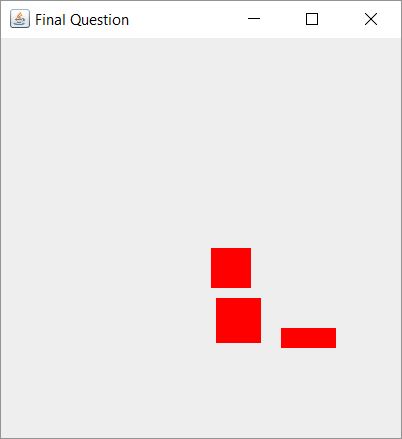
\includegraphics[width=0.32\linewidth]{stage1.PNG}
		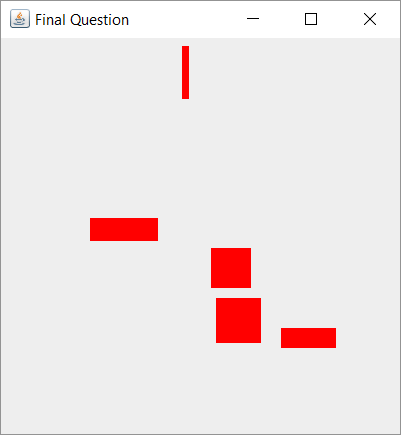
\includegraphics[width=0.32\linewidth]{stage2.PNG}
		\includegraphics[width=0.32\linewidth]{stage3.PNG}
	\end{center}
	\caption*{Stage 1 (left), Stage 2 (center), Stage 3 (right)}
	\label{fig:one}
\end{figure}


Read over all these instructions carefully.  Make sure you understand completely what functionality you have to implement before you start coding.  Ask questions if any part of the instructions are unclear.

\begin{itemize}
\item[Stage 1] (5 points) Uncomment the first block of code in \code{RectComponent}.  Your task is to add a new class, \code{RedRect}, that makes the given code work \textbf{(you should NOT modify the code in RectComponent)}.  

\code{RedRect's} constructor takes 4 parameters: x and y coordinates of the upper left corner of the rectangle, and the x and y coordinates of the lower right corner of the rectangle.  The draw function should draw a red filled rectangle - if you draw it correctly it will match the picture above.

\item[Stage 2] (6 points) Uncomment the second block of code in \code{RectComponent}.  Modify \code{RedRect} so the code works.  

When constructed with no parameters, the \code{RedRect} should have a random position with an upper left corner with x between 0 and 400 and y between 0 and 400.  The rectangle should have a random width and height between 0 and 100.  If you complete this code successfully, your picture will \textbf{not} exactly match the picture given but you should see random rectangles that change position/size when you resize the window.

\item[Stage 2] (6 points) Uncomment the third block of code in \code{RectComponent}.  Add a new class \code{RectContainer} to make the code work. 

\code{RectContainer}s have \code{RedRect}s added to them with an \code{addRect} method.  This method stores data so that when draw is called, the RectContainer should be a black outline exactly large enough to fit add of the rectangles that have been added to them.  You may have to add some methods to \code{RedRect} to make this possible.  

If you complete this code successfully, your picture will \textbf{not} exactly match the picture given, but both groups of rectangles should be exactly surrounded by a \code{RectContainer} outline.


\end{itemize}




\end{document}  
